\section{Hypotheses}

As noted in the first chapter, there are open questions regarding the efficiency of various gamified elements and how different genders relate to these gamified elements.
The question of the efficiency of certain elements and combinations of elements remains unresolved \parencite{dehghanzadehUsingGamificationSupport2024}.
To explore the connection between gender and gamification elements, we have created the following model:\newline

%\begin{tikzpicture}[node distance=0cm]
%    \tikzstyle{startstop} = [rectangle, minimum width=3cm, minimum height=1cm,text centered, draw=black, fill=red!30]
%    \tikzstyle{process} = [rectangle, minimum width=3cm, minimum height=1cm, text centered, draw=black, fill=orange!30]
%    \tikzstyle{arrow} = [thick,->,>=stealth]
%
%    \node (gender) [process] {Gender};
%    \node (gamified) [process, below left=2cm and 2cm of gender] {Gamified Elements};
%    \node (anxiety) [process, below right=0.2cm and 2cm of gender] {Anxiety};
%    \node (performance) [process, below=0.2cm of anxiety] {Performance};
%    \node (motivation) [startstop, below=0.2cm of performance] {Motivation};
%    \node (selfefficacy) [startstop, below=0.2cm of motivation] {Self efficacy};
%
%    \coordinate (MidPoint1) at ($(anxiety.west)!0.5!(selfefficacy.west)$);
%
%    % Calculate midpoint for the horizontal arrow
%    \coordinate (MidPoint2) at ($(gamified.east)!0.5!(MidPoint1)$);
%
%    \draw [arrow] (gamified) -- (MidPoint1);
%    \draw [arrow] (gender) -- (MidPoint2);
%\end{tikzpicture}\newline
\begin{figure}[H]
    \centering
    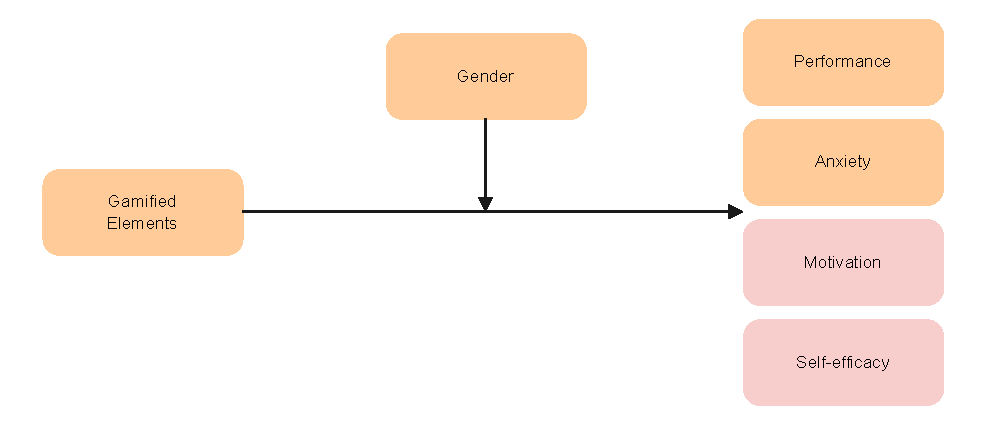
\includegraphics{img/Hypotheses}
    \label{fig:figureHypotheses}
\end{figure}
This model additionally incorporates concepts of motivation and self-efficacy, which, although not featured in my thesis, are included in the doctoral thesis of \textbf{Nadine Koch}.\newline
Since males perform better than females in solving progressive matrices from age 15 onward, Hypothesis \textbf{H1a} one-sidedly formulated \parencite{ravenStandardProgressiveMatrices2003}.
The hypotheses we want to investigate in this work are:
\begin{APAitemize}
    \item[H1] Males and females differ in their cognitive and affective states.
    \begin{APAitemize}
        \item[a)] Male performance is better compared to female.
        \item[b)] Male and female students differ regarding their anxiety levels.
        \item[c)] Male and female students differ regarding their motivation.
        \item[d)] Males have a higher self-efficacy compared to females.
    \end{APAitemize}
    \item[H2] Different gamified elements have a varying impact on the cognitive and affective states.
    \begin{APAitemize}
        \item[a)] Gamified elements impact performance differently.
        \item[b)] Different gamified elements impact anxiety levels differently.
        \item[c)] Different gamified elements impact motivation differently.
        \item[d)] Different gamified elements impact self-efficacy differently.
    \end{APAitemize}
    \item[H3] Different gamified elements differently impact the cognitive and affective states of males and females.
    \begin{APAitemize}
        \item[a)] The influence of different gamified elements on performance differs between males and females.
        \item[b)] The influence of different gamified elements on anxiety levels differs between males and females.
        \item[c)] The influence of different gamified elements on motivation differs between males and females.
        \item[d)] The influence of different gamification elements on self-efficacy differs between males and females.
    \end{APAitemize}
\end{APAitemize}
All hypothesized effects result from interacting with the gamified digital learning environment.